\chapter{Evaluation\label{cha:evaluation}}

In this chapter, the Orchestrator introduced in the previous chapter is tested and evaluated.
Although two use cases were presented in chapter \ref{cha:use-cases}, only the object detection application is evaluated here.
The sensor network use case was also tested with the system but is not described here because no additional findings were revealed.

In the first experiment, the nodes join and leave the network one after the other.
The second experiment investigates how the system behaves upon network quality changes.
For both experiments, the decisions the Orchestrator makes and the effect these decisions have on the total latency of the application are examined.




\section{Evaluation Setup}

\subsection{Infrastructure\label{sec:eval-infrastructure}}

\begin{figure}[htb]
    \centering
    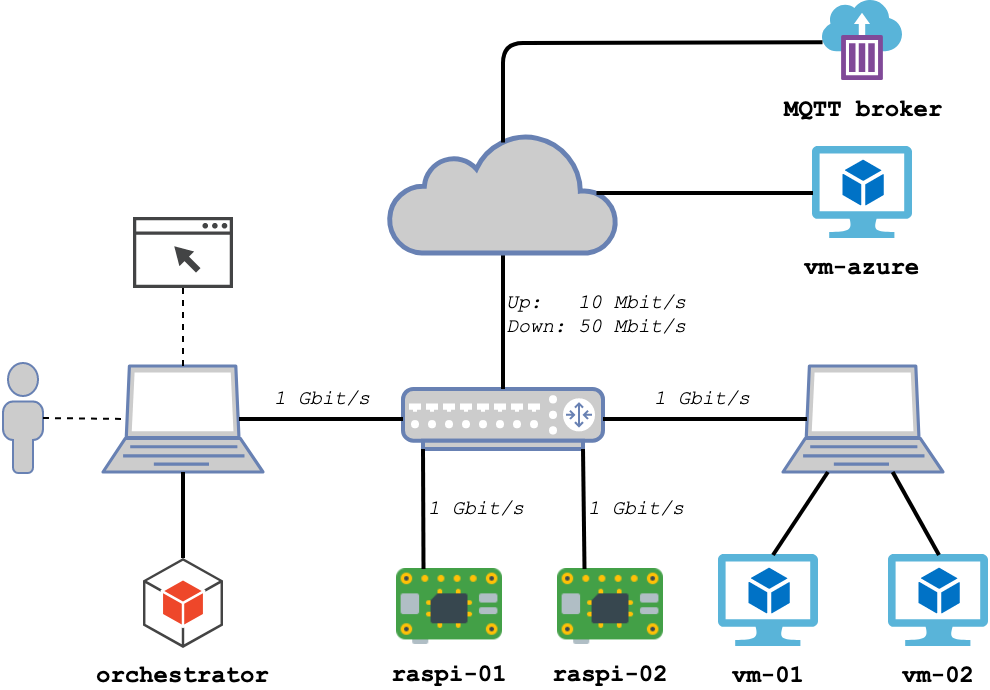
\includegraphics[width=0.85\textwidth]{evaluation-infrastructure}
    \caption{Test infrastructure for evaluation}
    \label{fig:evaluation-infrastructure}
\end{figure}

\begin{table}[htb]
    \centering
    \begin{tabular}{|l|l|l|l|l|l|}
    \hline
        \textbf{Node} & \textbf{Device Type} & \textbf{CPU} & \textbf{RAM} \\
         \hline
         \texttt{raspi-01} & Raspberry Pi 3B+ & ARM Cortex-A53 1.4 GHz, 4 cores & 1 GB\\
         \hline
         \texttt{raspi-02} & Raspberry Pi 4B & ARM Cortex-A72 1.5 GHz, 4 cores & 4 GB\\
         \hline
         \texttt{vm-01} & Hyper-V VM & Intel i7-8550U 1.8 GHz, 2 vCPUs & 2 GB\\
         \hline
         \texttt{vm-02} & Hyper-V VM & Intel i7-8550U 1.8 GHz, 4 vCPUs & 4 GB\\
         \hline
         \texttt{vm-azure} & Azure VM \texttt{F4s\_v2} & Intel Xeon 2.7 GHz, 4 vCPUs & 8 GB\\
         \hline
    \end{tabular}
    \caption{Hardware characteristics of test devices used for evaluation}
    \label{tab:evaluation-devices}
\end{table}

The test bed consists of the five nodes presented in figure \ref{fig:evaluation-infrastructure}. The hardware characteristics of the devices are shown in table \ref{tab:evaluation-devices}. The two Raspberry Pis run Raspbian 10, the three virtual machines run Debian 10. All nodes have \texttt{Docker version 19.03.2} installed. Another device on the local network runs the Orchestrator and a web browser which is used to access the \textit{Object Detection Web Application}. Communication between the nodes and the Orchestrator is done via a MQTT broker running in the Azure Cloud.

\subsection{Application\label{sec:eval-application}}

\begin{figure}[htb]
    \centering
    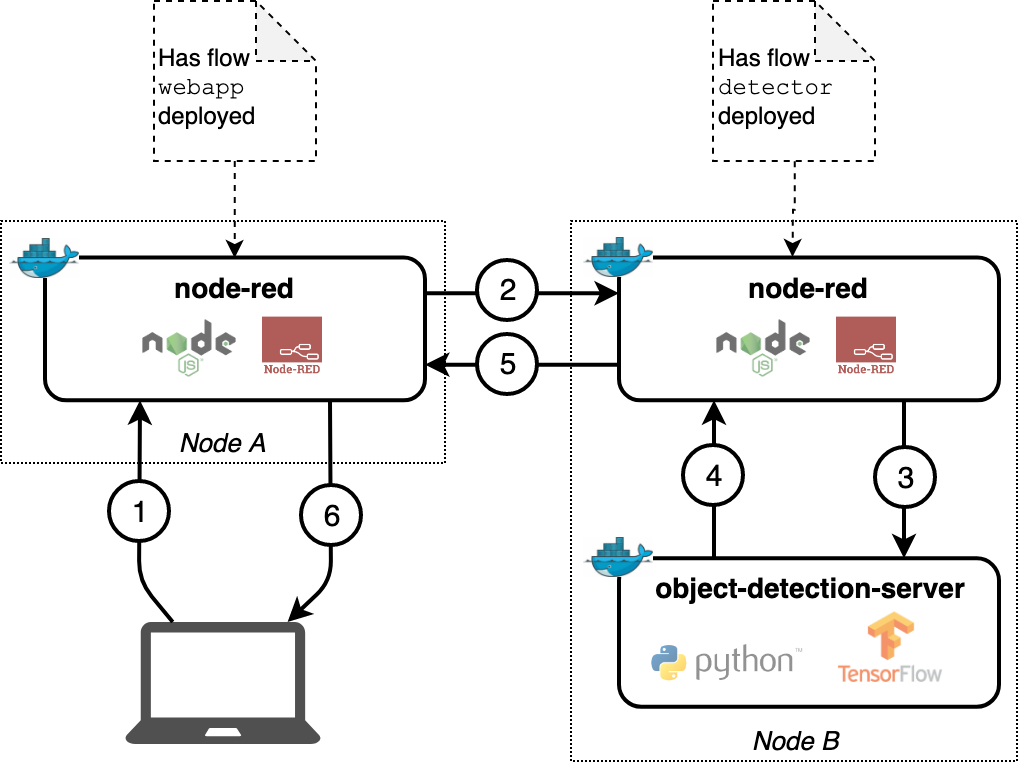
\includegraphics[width=0.85\textwidth]{evaluation-application}
    \caption{System architecture of the Object Detection Web Application}
    \label{fig:evaluation-object-detection-application}
\end{figure}

The \textit{Object Detection Web Application} consists of the two modules \texttt{webapp} and \texttt{detector} as illustrated in figure \ref{fig:evaluation-object-detection-application}.
A screenshot of the web application is shown in figure \ref{fig:object-detection-webapp-screenshot}.\\

In the first step, a user sends an image for object detection to the \texttt{webapp} module which is deployed as a Node-RED flow on \texttt{Node A}.
This module should always be deployed on the same node and not be moved, so that the web application is always available at the same address.
The user calls the web application on that fixed node while it is irrelevant for him which node actually executes the object detection task.
The module \texttt{webapp} forwards the image to the module \texttt{detector} for object detection which is deployed on another node (\texttt{Node B}).
This node can vary and is chosen by the Orchestrator.
If a new node is selected by the Orchestrator, the flow \texttt{webapp} on \texttt{Node A} will then be updated so that subsequent requests are forwarded to the new node.\\

The object detection engine cannot be executed as a regular Node-RED flow since Node-RED handles JavaScript functions only and the engine requires Python.
Even if Node-RED could execute Python code (there are extensions enabling this), the execution of the object detection engine in Node-RED would not be efficient because the engine would have to be initialized every time a new object detection request arrives.
However, the engine has a certain initialization time to load the detection graph. Therefore it is more efficient to initialize the engine only once at the beginning so that the following object detection tasks can be executed without additional initialization time. Because Node-RED cannot initialize and hold Python objects, a separate Docker container is used for this purpose. The flow \texttt{detector} sends an HTTP request containing the undetected image to the \texttt{object-detection-server} running on the same node. The server responds with the detected image which the \texttt{detector} then sends back to the \texttt{webapp} module.

The following three constraints are defined for the experiment:
\begin{enumerate}
    \item The flow \texttt{webapp} must be deployed on \texttt{raspi-01} because this is the only node known to the user
    \item The flow \texttt{detector} needs an \texttt{object-detection-server} Docker container running on the same node which is the case for all nodes except for \texttt{raspi-01}
    \item The detected image must be available within 5 seconds
\end{enumerate}








\section{Preparing the Orchestrator\label{sec:eval-preparing-the-orchestrator}}

For evaluating the Orchestrator, nodes with different CPU's performance are necessary.
However, one vCPU in \texttt{vm-01} is equally as fast as in \texttt{vm-02} because they both run on the same host.
Since the object detection engine uses only one core, the execution time on these two nodes is approximately the same, although \texttt{vm-01} has two cores and \texttt{vm-02} has four cores.
For this reason, the Docker containers on \texttt{vm-01} run with the additional option \texttt{---cpus="0.5"} which limits the available CPU resources a container can use to a half vCPU.

\clearpage
\subsection{Possible Deployment Strategies\label{sec:eval-possible-deployments}}

\begin{figure}[h!]
    \centering
    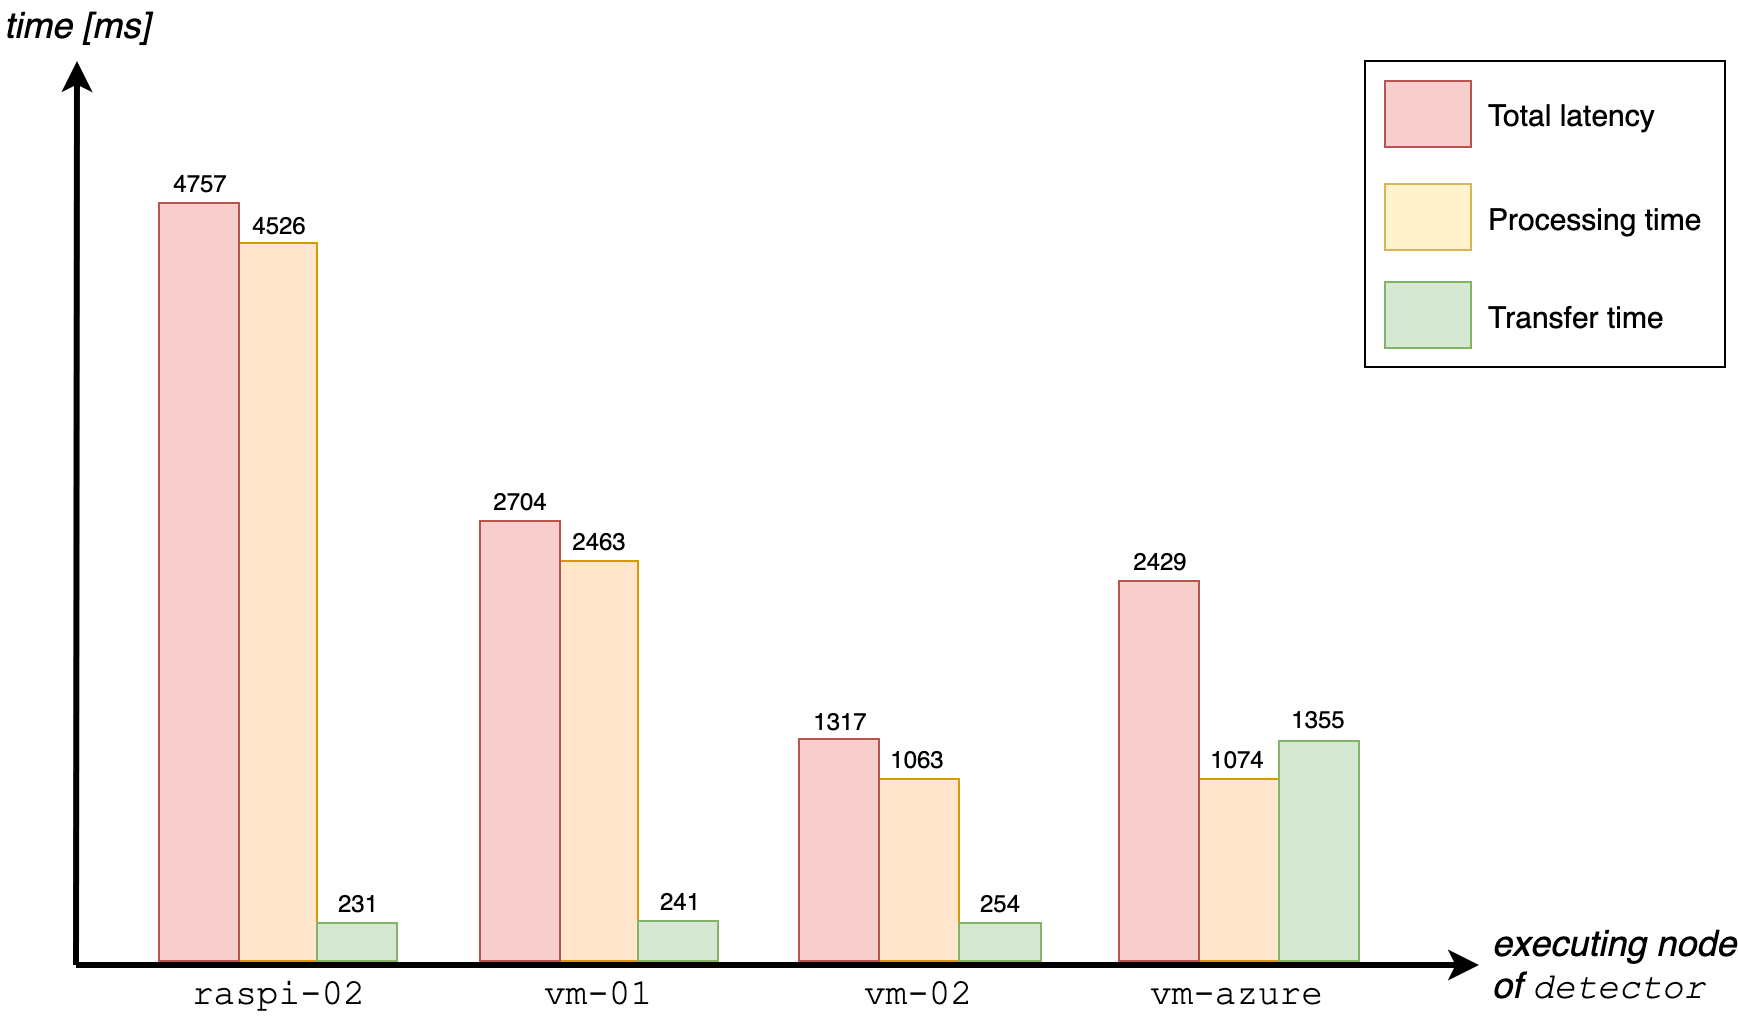
\includegraphics[width=1.0\textwidth]{evaluation-total-latency-without-orchestrator}
    \caption{Total latencies, execution times, and transfer times of the object detection application regarding the placement of module detector}
    \label{fig:evaluation-total-latency-without-orchestrator}
\end{figure}

To find the actual execution times of all possible deployment strategies, the application was deployed to the infrastructure without using the Orchestrator.
The module \texttt{webapp} was always deployed on node \texttt{raspi-01} while the module \texttt{detector} was switched through the remaining nodes.
The object detection application was executed 10 times on each deployment strategy by using a 1,383 KB sized image.
The mean values for \textit{total latency}, \textit{processing time} and \textit{transfer time} were calculated thereafter. These are compared in figure \ref{fig:evaluation-total-latency-without-orchestrator}.
Based on the measurement results, a prioritization of all possible deployments was created where deployments with a lower latency were preferred (see table \ref{tab:deployment-strategies-prios}).

\begin{table}[h!]
    \centering
    \begin{tabular}{|l|l|l|l|l|l|}
    \hline
        \textbf{Priority} & \textbf{Placement of \texttt{webapp}} & \textbf{Placement of \texttt{detector}} & \textbf{Latency} \\
         \hline
         \texttt{1} & \texttt{raspi-01} & \texttt{vm-02} & 1,317 ms\\
         \hline
         \texttt{2} & \texttt{raspi-01} & \texttt{vm-azure} & 2,429 ms\\
         \hline
         \texttt{3} & \texttt{raspi-01} & \texttt{vm-01} & 2,704 ms\\
         \hline
         \texttt{4} & \texttt{raspi-01} & \texttt{raspi-02} & 4,757 ms\\
         \hline
    \end{tabular}
    \caption{Possible deployment strategies for the object detection application}
    \label{tab:deployment-strategies-prios}
\end{table}

\subsection{Defining the Application\label{sec:eval-defining-application}}

Although the Orchestrator handles the infrastructure dynamically, an application must be defined. 
Therefore, an \texttt{Application} object is created during the initialization of the Orchestrator.
It contains all modules, loops and messages of the object detection application described in section \ref{sec:eval-application}.

\subsubsection*{Setting required RAM and disk storage}
The fields \texttt{requiredRam} and \texttt{requiredStorage} of the two modules \texttt{webapp} and \texttt{detector} are set to \texttt{0} because both Node-RED flows are relatively small and thus consume neither significant RAM nor storage.
Although the \texttt{object-detection-server} container requires 1GB RAM, this memory is not allocated/released by deploying/removing the flow to/from Node-RED because the container runs even if the Node-RED flow is not deployed on a node.
Furthermore, the container does not require any additional disk storage while running the engine.

\subsubsection*{Setting required hardware modules}
The field \texttt{requiredHardwareModules} of the module \texttt{webapp} contains one string: \texttt{"CAMERA"}.
The \texttt{node-red} Docker container on \texttt{raspi-01} is started with the additional option \texttt{-e CONNECTED\_HARDWARE=["CAMERA"]} so that \texttt{webapp} can only be deployed on \texttt{raspi-01}. The same approach is used for the module \texttt{detector}, but here the string \texttt{"OD-DOCKER-CONTAINER"} is used and passed to the Docker container on the remaining nodes instead.

\subsubsection*{Setting required instructions}
The field \texttt{requiredMi} of the module \texttt{webapp} is set to \texttt{0} because the Node-RED flow simply forwards messages and therefore does not require any significant CPU power.
However, CPU resources consumed by the module \texttt{detector} are substantial.
Since the Orchestrator uses a CPU score instead of MIPS, the value for \texttt{requiredMi} has to be calculated using the formula introduced in section \ref{sec:benchmark-cpu}.
Values for \textit{CPU score} and \textit{execution time} are taken from \texttt{vm-02}, which are \textit{11,661} and \textit{1,317 ms}, respectively.
Therefore:
\[\textrm{\texttt{requiredMi\textsubscript{detector}}} = \textrm{CPU score} \boldsymbol{\cdot} \frac{\textrm{execution time [ms]}}{1,000 \textrm{ [ms]}} = 11,661 \boldsymbol{\cdot} \frac{1,317}{1,000} = 15,357\]

\subsubsection*{Setting the loop and messages}
The application has exactly one loop (instance of \texttt{AppLoop}) where the field \texttt{modules} is populated with a list containing three elements in the following order:
\texttt{"webapp"}, \texttt{"detector"}, \texttt{"webapp"}.
The field \texttt{maxLatency} is set to \texttt{5000}.

Furthermore, the application contains two messages (instances of \texttt{AppMessage}).
The first one contains the original image, which in this case has a file size of 1,383 KB. Therefore, the fields \texttt{contentType} and \texttt{dataPerMessage} are set to \texttt{"IMAGE\_UNDETECTED"} and  \texttt{1383}, respectively. This is the input message to the module \texttt{detector}.
The second message contains the detected image, which has a file size of 142 KB. Therefore, the fields are set to \texttt{"IMAGE\_DETECTED"} and \texttt{142}, respectively. This is the output message of the module \texttt{detector}.









\section{Experiment 1: Consistent Network Quality\label{sec:eval-exp-1}}

In this experiment, the nodes were started in the following order:
\begin{enumerate}
    \item \texttt{raspi-01}
    \item \texttt{raspi-02}
    \item \texttt{vm-01}
    \item \texttt{vm-azure}
    \item \texttt{vm-02}
\end{enumerate}
This order allows to apply the deployment strategy of lowest priority (priority four) in step two, while a strategy of higher priority is possible with each following step (see table \ref{tab:deployment-strategies-prios}).

It was expected that the Orchestrator finds no valid deployment in step one because solely \texttt{raspi-01} is online which is unable to execute the module \texttt{detector}.
Another expectation was that the Orchestrator deploys the module \texttt{webapp} to \texttt{raspi-01} and \texttt{detector} to \texttt{raspi-02} in the second step and then moves the \texttt{detector} to \texttt{vm-01}, \texttt{vm-azure} and finally to \texttt{vm-02} in the subsequent steps, while \texttt{webapp} remains on \texttt{raspi-01}.

\subsection*{Results}

\begin{figure}[htb]
    \centering
    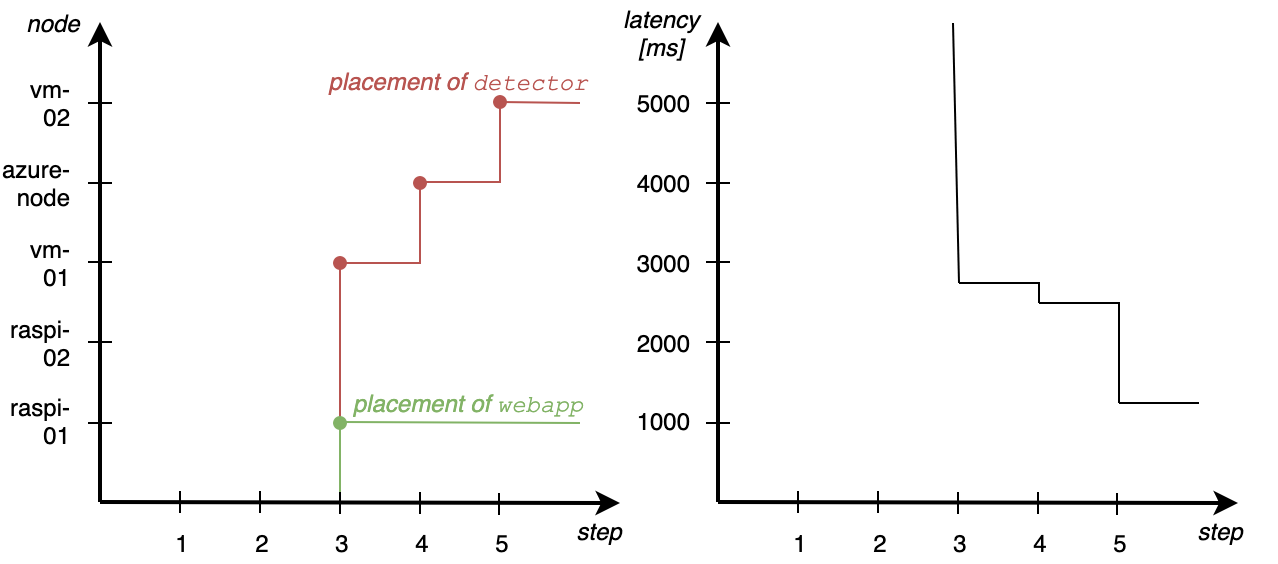
\includegraphics[width=1.0\textwidth]{evaluation-exp1-result}
    \caption{Result of Experiment 1: Orchestrator's decisions and their impact on total latency}
    \label{fig:evaluation-exp1-results}
\end{figure}

The Orchestrator's decisions are depicted in figure \ref{fig:evaluation-exp1-results}.
The figure shows that the Orchestrator behaved slightly different than expected.
The \texttt{detector} was expected to be deployed to \texttt{raspi-02} in the second step. However, this did not happen.
Instead, no possible deployment was found.
In steps 1, 3, 4 and 5, however, the Orchestrator made the expected decisions and the latency is minimized continuously from step 3 onwards.

Moreover, it was examined how the Orchestrator behaves when a node leaves the network.
If a node that has \textit{no} module deployed leaves the network, the Orchestrator detects this and removes it from the infrastructure.
The deployment strategy remains unchanged as it should be.
If a node that \textit{has} a module deployed leaves the network, the Orchestrator detects this and removes it from the infrastructure first before it then finds and applies the next best possible deployment strategy (next best deployment strategy is the one of highest priority in the updated infrastructure).
This complies with the desired behaviour.

\subsection*{Investigation of the Orchestrator's incorrect decision\label{sec:eval-investigation-cpu}}

The reason for the wrong decision in step two is that the execution time of module \texttt{detector} on node \texttt{raspi-02} calculated by the Orchestrator is incorrect.
The field \texttt{cpuMips} of the \texttt{FogNode} object representing this node has the value 973.
This value is the CPU score returned by the \texttt{benchmark\_cpu} command which the Orchestrator executed on the node after the first heartbeat has been received (see section \ref{sec:handling-new-fog-nodes} and \ref{sec:benchmark-cpu} in particular).
To calculate the execution time of module \textit{M} on node \textit{N}, the Orchestrator uses \texttt{cpuMips} of \textit{N} and \texttt{requiredMi} of \textit{M}.
While preparing the Orchestrator in section \ref{sec:eval-preparing-the-orchestrator}, \texttt{requiredMi\textsubscript{detector}} was set to 15,357. Thus, the execution time is calculated as follows:

\[\textrm{execution time [ms]} = \frac{\textrm{\texttt{requiredMi}}}{\textrm{\texttt{cpuMips}}}\ \boldsymbol{\cdot} 1,000 = \frac{15,357}{973}\ \boldsymbol{\cdot} 1,000 = 15,783 \textrm{ [ms]}\]

The calculated execution time is approximately 3.5 times greater than actual execution time of 4,526 milliseconds (see figure \ref{fig:evaluation-total-latency-without-orchestrator}).
Furthermore, it is greater than 5,000 milliseconds, which is the \texttt{maxLatency} of the opject detection loop. 
Therefore, the Orchestrator finds no valid deployment strategy.

The \texttt{benchmark\_cpu} command internally uses the CPU benchmarking tool \texttt{sysbench} which searches for all prime numbers between 1 and a certain upper limit (2000 in this case) and returns the time needed to execute this task.
Apparently, this time cannot be used to deduce the execution time of other types of tasks like object detection.
To further investigate this, the simple JavaScript function shown in listing \ref{lst:simple-javascript-function} was executed in Node-RED on \texttt{raspi-02} and \texttt{vm-02} while no other CPU intensive processes were running.

\begin{lstlisting}[language=JavaScript,numbers=none,caption={JavaScript function which executes simple mathematical tasks while measuring the total execution time},label=lst:simple-javascript-function]
const timeStart = new Date();
let result = 0;
for (let i=0; i < Math.pow(10,7); i++) {
    result = result + i;
}
const timeEnd = new Date();
const time = timeEnd - timeStart;
\end{lstlisting}

The field \texttt{time} of that function contains the execution time in milliseconds which is approximately 2,500 on \texttt{vm-02} and 7,500 on \texttt{raspi-02}, respectively. 
Thus, the execution of the function is about \textit{3 times faster} on \texttt{vm-02} than on \texttt{raspi-02}, even though the CPU score of \texttt{vm-02} (11,848) is about \textit{12 times greater} than the score of \texttt{raspi-02} (973).
Additionally, the object detection task takes about 1,063 milliseconds on \texttt{vm-02} and 4,757 milliseconds on \texttt{raspi-02}, which is a \textit{4,2-fold difference} (see figure \ref{fig:evaluation-total-latency-without-orchestrator}).
Therefore, a correlation between the execution times of different tasks on various nodes cannot be recognized.

However, there might be a correlation between CPUs that share the same architecture, but this is not the case either:
Executing the function shown in listing \ref{lst:simple-javascript-function} takes about 17,800 milliseconds on \texttt{raspi-01}, which is \textit{2.37 times slower} than on \texttt{raspi-02}, although the CPU score of \texttt{raspi-01} (612) is only \textit{1.59 times smaller} than on \texttt{raspi-02}. Both nodes own a CPU of type \texttt{arm}.\\

In conclusion, the execution time of a given task cannot be used as the basis to compare CPU performances of different devices.
There seem to be a number of relevant factors affecting the execution time of a task, but this goes beyond the scope of this work.




\section{Experiment 2: Volatile Network Conditions}

In this experiment, the three nodes \texttt{raspi-01}, \texttt{vm-01} and \texttt{vm-azure} were online. Therefore, deployment strategy of \textit{priority two} allowed the lowest latency (see table \ref{tab:deployment-strategies-prios}).
Here, the \texttt{detector} module is deployed on \texttt{vm-azure}.
In further course, the router's internet connection was utilized by other hosts on the network that are not part of the fog infrastructure.
After a certain period, the bandwidth was freed again.


It was expected that the Orchestrator moves the \texttt{detector} module from \texttt{vm-azure} to \texttt{vm-01} after the usage of the internet connection exceeds a certain threshold.
This is the case as soon as the application no longer has enough bandwidth to meet its latency requirements.
After the full bandwidth is available again, the \texttt{detector} should be moved back to \texttt{vm-azure} by the Orchestrator as soon as possible.


\subsection*{Results}

\begin{figure}[htb]
    \centering
    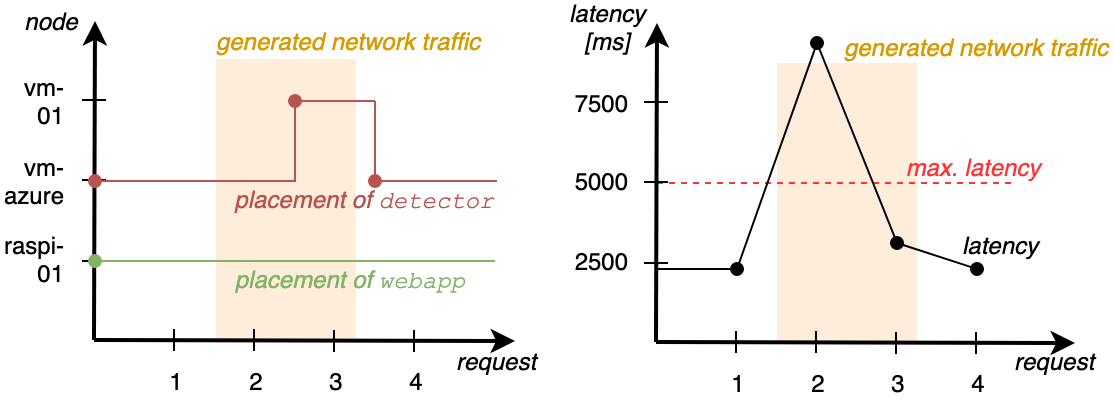
\includegraphics[width=1.0\textwidth]{evaluation-exp2-result}
    \caption{Result of Experiment 2: Orchestrator's decisions and their impact on total latency}
    \label{fig:evaluation-exp2-results}
\end{figure}

The Orchestrator's decisions are depicted in figure \ref{fig:evaluation-exp2-results}. 
Initially, it applied deployment strategy of priority two as expected.
The object detection task in request one was finished after 2,370 milliseconds, while the \texttt{detector} was executed on \texttt{vm-azure}.

Between request one and two, network traffic between a host in the local network and another host on the internet was generated.
Both hosts were not part of the fog infrastructure, but they did utilize the same internet connection that was used for transferring the original image from \texttt{webapp} (deployed on \texttt{raspi-01}) to \texttt{detector} (deployed on \texttt{vm-azure}) as well.
That is why the maximum latency requirement of 5,000 milliseconds could not be met in request two.
Although the object detection task on \texttt{vm-azure} took approximately the same time in both requests, the time for transferring the original image (1,382 KB) took 7,641 milliseconds instead of 1,192 milliseconds in request one, so that the total latency added up to 8,921 milliseconds.

The Orchestrator recognized this by evaluating the \texttt{statistics} object (see listing \ref{lst:statistics}) introduced in section \ref{sec:orchestrator-monitoring-deployment-strategy}.
Based on the image size and transfer time, it calculated the actual bandwidth between both nodes, which is \textit{1.48 Mbit/s} in this case.
The respective \texttt{NetworkUplink} object was updated and the scheduling algorithm was executed to find a new optimal deployment strategy.
This is what happened between request two and three, before the \texttt{detector} was moved to \texttt{vm-01}.
The latency requirement was fulfilled in request three, although the total latency of 2,671 milliseconds is a bit higher than in request one.

As said before, the scheduling algorithm was triggered during the evaluation of the \texttt{statistics} object in this case.
However, the Orchestrator executes the algorithm in a predefined interval as well.
Since the uplinks are also remeasured in a predefined interval by the Orchestrator, the scheduling algorithm might find a new optimal deployment strategy.
This is what happened between request three and four:
The network traffic generation has been stopped and the uplink between \texttt{raspi-01} and \texttt{vm-azure} has been remeasured.
The updated bandwidth was taken into account during the subsequent execution of the scheduling algorithm, so that the Orchestrator switched back to the deployment strategy of priority two which led to a lower latency in request four.

It should be added that there might be a new optimal deployment strategy in case of a downgrade of an uplink, even though the new strategy might have a higher latency than the previous one.
This could be the case if an uplink that is involved in the current deployment strategy deteriorates.
Nevertheless, the Orchestrator always applies the deployment strategy which allows the lowest latency to the best of his knowledge.


\clearpage
\section{Discussion}

The evaluation showed that the Orchestrator developed in this thesis is fundamentally able to dynamically apply different deployment strategies to a Node-RED environment resulting in an optimized quality of service.

The measurements of the network connections between the nodes produced realistic results, to that the Orchestrator could estimate transfer times of messages fairly well.
Calculating the execution time of tasks has partly delivered unrealistic results, so this estimation does not work reliably and can lead to wrong decisions as happened in the first experiment.
The reason for this is the method used by the Orchestrator to measure and compare the CPU performance of different devices.
A program is run on every new fog node joining the infrastructure, while the execution time is measured.
However, the execution time of one task cannot be set in relation to the execution time of another task.

In the first experiment, the values of \texttt{vm-02} were used as the basis for calculating \texttt{requiredMi\textsubscript{detector}}.
Therefore, the execution time of the \texttt{detector} module could be calculated relatively precisely on \texttt{vm-02}.
The same was true for \texttt{vm-01}, since both nodes shared the same CPU, although the CPU of \texttt{vm-01} was limited.
If the values of \texttt{raspi-02} had been used to calculate \texttt{requiredMi\textsubscript{detector}} instead, the execution time of \texttt{detector} on \texttt{raspi-02} would have been estimated correctly, but the estimated execution time on other nodes would have been wrong.

In the second experiment, the deployment strategy changed \textit{after} failing to process a request within the required time.
This could have been avoided by setting lower intervals for checking uplinks and deployment strategies, thus the increased network traffic after request one would have been detected earlier.
Therefore, the Orchestrator would have changed the deployment strategy \textit{before} request two, so the maximum allowed latency would not have been exceeded.
However, the uplink measurements generate network traffic themselves, so that this interval should be chosen with caution.
If set too low, the measurements would constantly use bandwidth, thus leading to higher latency of the deployed services.

Although the system enables the QoS-aware task execution on distributed Node-RED clusters, there are some expansion and improvement capabilities of the system which are discussed in the next and last chapter.